\documentclass{standalone}

\usepackage{tikz,pgf} %and any other packages or tikzlibraries your picture needs

\usepackage{pgfplots}

\usepackage[utf8]{inputenc}
\usepackage[colorlinks=true, allcolors=blue]{hyperref}
\usetikzlibrary{positioning, arrows.meta, fit, shapes}
\begin{document}

    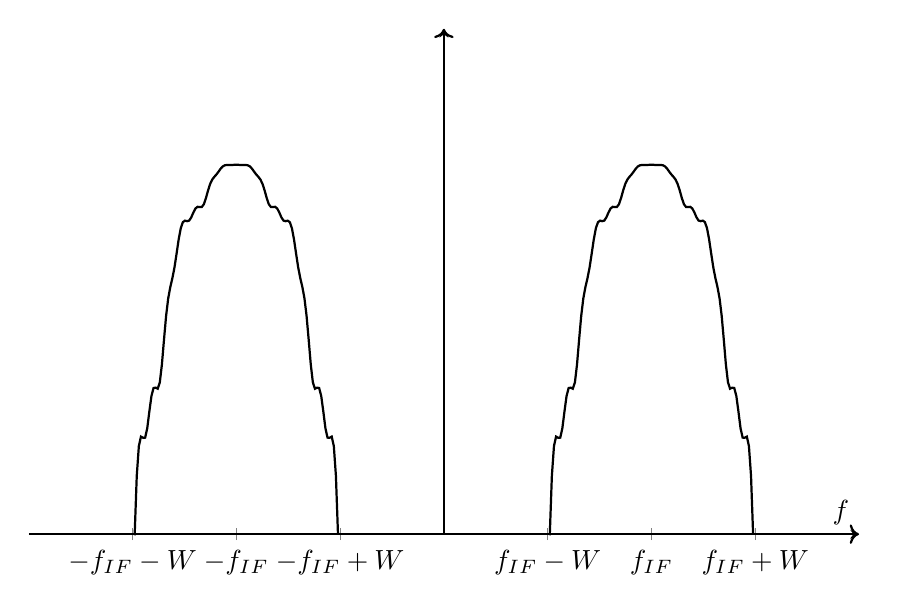
\begin{tikzpicture}
        \begin{axis}[
            axis lines=middle,
            width=\textwidth,
            height=8cm,
            xlabel={$f$},
            ylabel={},
            xtick={-3,-2,-1,0,1,2,3},
            xticklabels={$-f_{IF}-W$, $-f_{IF}$, $-f_{IF}+W$, $0$, $f_{IF}-W$, $f_{IF}$, $f_{IF}+W$},
            ytick=\empty,
            xmin=-4,
            xmax=4,
            ymin=0,
            ymax=1,
            clip=false
        ]

        \pgfmathsetmacro{\fIF}{2}
        \pgfmathsetmacro{\W}{1}

        \addplot[domain=-\fIF-\W:-\fIF+\W, samples=100, black, thick] 
            ({x}, {((sqrt(-15129*(x+\fIF)^2 + 1968*(x+\fIF)*sin(deg(15*(x+\fIF)))^3 - 64*sin(deg(15*(x+\fIF)))^6 + 14400))/(120))} - 0.269 );
        \addplot[domain=\fIF-\W:\fIF+\W, samples=100, black, thick] 
            ({x}, {((sqrt(-15129*(x-\fIF)^2 + 1968*(x-\fIF)*sin(deg(15*(x-\fIF)))^3 - 64*sin(deg(15*(x-\fIF)))^6 + 14400))/(120))} - 0.269 );

        \draw[->,thick] (axis cs:-4,0) -- (axis cs:4,0) node[right] {};
        \draw[->,thick] (axis cs:0,0) -- (axis cs:0,1);

        \end{axis}
    \end{tikzpicture}

\end{document}
